\documentclass[../IND E 315.tex]{subfiles} 
\usepackage{fancyhdr}
\usepackage{graphicx}
\usepackage{amsmath}
\usepackage{mhchem}
\usepackage{amssymb}
\usepackage[margin=1in]{geometry}

\usepackage{subfiles} % Best loaded last in the preamble
\graphicspath{{./images/}}

\title{UW IND E 315 Notes}
\author{Anthony Le}

\newtheorem{exmp}{Example}
\newtheorem{exrc}{Excersize}
\newtheorem{proof}{Statement}
\newtheorem{defn}{Definition}


\begin{document}

\pagestyle{fancy}
\fancyhead{}
\fancyhead[R]{UW IND E 315}
\fancyhead[L]{Anthony Le}

\section*{Chapter 2 - Probability}
\subsection*{Simple Example}
\begin{exmp}
    What is the probability of getting heads on the toss of a coin?
\end{exmp}
\begin{defn}
    \textbf{Probability} \\
    The likelihood of a particular outcome/event.
    \begin{enumerate}
        \item Formally: a number from the interval [0,1] to indivate the low (0) to high (1) likelihood of occurrence.
    \end{enumerate}
\end{defn}

\begin{defn}
    \textbf{Sample Space} \\
    The set of all possible outcomes of a random experiment.
    \begin{enumerate}
        \item Event: Subset of the sample space
    \end{enumerate}
\end{defn}

\subsection*{Sample Space and Event (2.1)}
\begin{center}
    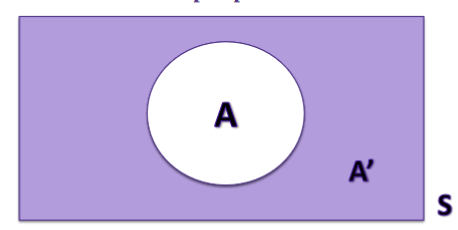
\includegraphics{Example2.1}
\end{center}
Given a sample space $S$ where the probability of S is 1, you can find the probability of event $A$ by subtracting the probability of $A'$ from the probability of the sample space. Describing this in math terms:
\begin{equation*}
    \begin{aligned}
        \text{Sample Space where } P(S) = 1 \\
        P(A) = 1- P(A')
    \end{aligned}
\end{equation*}

\begin{exmp}
    What is the example space for the sum of 2 dice?
\end{exmp}
\begin{equation*}
    \begin{aligned}
        S = {2,3,4,5,6,7,8,9,10,11,12}
    \end{aligned}
\end{equation*}
\begin{enumerate}
    \item Let A be the event that the dice rolls an even number:
        \begin{equation*}
            \begin{aligned}
                A = {2,4,6,8,10,12}
            \end{aligned}
        \end{equation*}
    \item Let B be the event that the dice rolls a prime number:
        \begin{equation*}
            \begin{aligned}
                B = {2,3,5,7,11}
            \end{aligned}
        \end{equation*}
\end{enumerate}
From this, find these following:
\begin{enumerate}
    \item $P(A) = ?$
    \item $P(B) = ?$ 
    \item $P(A|B) = ?$
\end{enumerate}

Here's a graphic showing the sample space for the above situation:
\begin{center}
    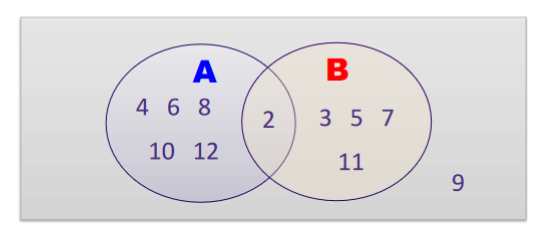
\includegraphics{Ch2Example2}
\end{center}
To find $P(A|B)$:
\begin{equation*}
    \begin{aligned}
        P(A|B) = \frac{P(A \cap B)}{P(B)}
    \end{aligned}
\end{equation*}

\subsection*{Interpretations and Axioms of Probability (2.3)}
\begin{enumerate}
    \item Let S be the sample space of some random experiment.
    \item Let E be some event within that sample space.
    \item $P(E)$, the probability of the event is \emph{assigned} based on our knowledge of the system under study.
    \item \emph{Mathematically}, $P(E)$ should satisify the three axioms of probability.
        \begin{enumerate}
            \item The axioms ensure that:
                \begin{enumerate}
                    \item The assigned probabilities can be \emph{interpreted as relateive frequencies}
                    \item The assignments are \emph{consistent with our intuitive understanding} of relationships between relative frequencies.
                \end{enumerate}
        \end{enumerate}
\end{enumerate}

\subsubsection*{Axioms of Probability}
\begin{enumerate}
    \item $0 <= P(E) <= 1$ for any event E.
    \item $P(S) = 1$ where $S$ is the sample space.
    \item If $E_1$, $E_2$,... are mutually exclusive events (ex $E_1 \cap E_2 = 0$), then $P(E_1 \cup E_2) = P(E_1) + P(E_2)$.
\end{enumerate}

\subsection*{Event: subset of the sample space - combination of events}
%tags - tag vs cup, union, intersection
\begin{enumerate}
    \item Union of two events
        \begin{enumerate}
            \item All events are contained in \emph{either} of the two events
            \item Denoted at $E_1 \cup E_2$
        \end{enumerate}
        \begin{center}
            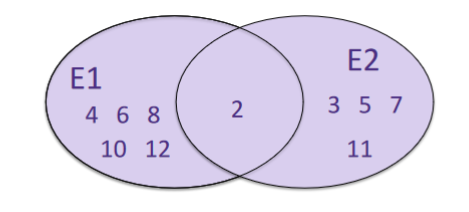
\includegraphics[width = 5cm]{Ch2Event_Union}
        \end{center}
\end{enumerate}





\end{document}